\documentclass[xetex,mathserif,serif]{beamer}

\usepackage[log-declarations=false]{xparse}
\usepackage[quiet]{fontspec}
\usepackage{amsmath}
\usepackage{amsfonts}
\usepackage{mathtools}
\usepackage{enumerate}
\usepackage{polyglossia}
\usepackage{tikz}
\usepackage{unicode-math}
\usetikzlibrary{arrows,shapes,trees}

\newcommand{\vank}{\emph{Seifert-van Kampen} }

% works for now
\setbeamertemplate{footline}{\insertframenumber/\inserttotalframenumber}

\setdefaultlanguage{spanish}

\begin{document}

  \begin{frame}
    \begin{block}{}
      \centering
      Topología Algebraica
    \end{block}
    \begin{block}{}
      \centering
      Rubén Astudillo Colina
    \end{block}

  \end{frame}

  \begin{frame}
    \frametitle{Motivación}

    \begin{block}{}
      Definir una invariante para espacios topológicos.
    \end{block}

    \pause

    \begin{block}{}
      Idea: Estudiar las curvas y las ``deformaciones'' admisibles entre
      ellas para un espacio dado.
    \end{block}
  \end{frame}

  \begin{frame}
    \frametitle{Curvas y homotopías}
    \begin{columns}

      \begin{column}{.5\textwidth}
        \begin{center}
          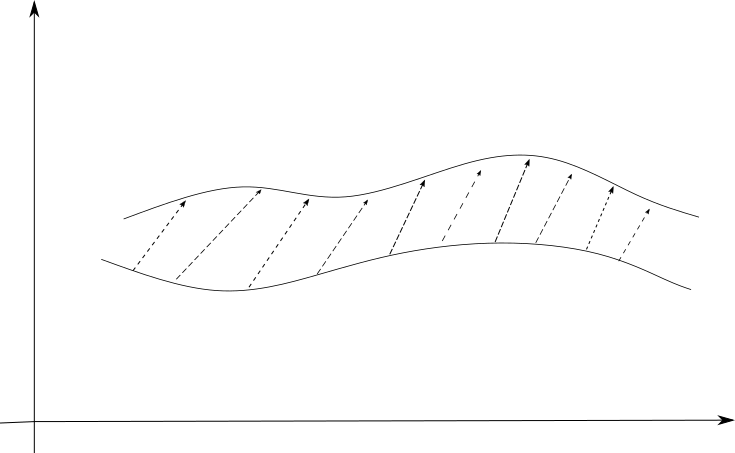
\includegraphics[scale=0.3]{../tesis/imagenes/homotopia.png}
        \end{center}
      \end{column}

      \begin{column}{.5\textwidth}
        \begin{block}{Camino}
          Es una función continua \[ f : I \to X \] con \(X\) un espacio
          topológico
        \end{block}

        \begin{block}{Homotopía entre \(f\) y \(g\)}
          Es una función continua \(H : I \times I \to X\) tal que
          \[ H(x,0) = f(x),\ H(x,1) = g(x) \]
          \[ f \sim g \]
        \end{block}
      \end{column}
    \end{columns}
  \end{frame}

  \begin{frame}
    \frametitle{Producto de caminos y homotopías}
    Si \(f (1) = g (0) \in X\) entonces el producto de caminos esta
    definido por
    \[ f * g (t) :=
      \begin{cases}
        f(2t) & t \in [0, \frac 1 2] \\
        g(2t - 1) & t \in [\frac 1 2 , 1 ]
      \end{cases}
    \]

    \begin{center}
      \begin{tikzpicture}[scale=0.8]
        \draw [blue, thick]  (0,0) to[bend right] (3,2) to[bend left] (4,3) ;
        \draw [red, thick] (4,3) to[bend right] (9,1) ;
      \end{tikzpicture}
    \end{center}

    \pause

    \begin{block}{}
      En general se consideran curvas con el mismo punto inicial y final
      (caminos cerrados).
    \end{block}
  \end{frame}

  \begin{frame}
    \frametitle{Producto de caminos y homotopías}
    Análogamente para homotopías \(F\) y \(G\) tal que \(H(1, t) =
    G(0,s) , \forall s, t \in I\), se define el producto de homotopías
    \[ F * G (x, t) :=
      \begin{cases}
        F(x, 2t) & t \in [0, \frac 1 2] \\
        G(x, 2t - 1) & t \in [\frac 1 2, 1]
      \end{cases}
    \]

    \begin{center}
      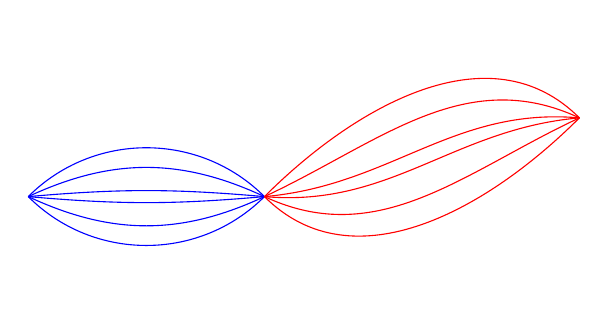
\begin{tikzpicture}
        \draw[blue] (0,1) to[out=45, in=135] (3,1) ;
        \draw[blue] (0,1) to[out=25, in=155] (3,1) ;
        \draw[blue] (0,1) to[out=5, in=175] (3,1) ;
        \draw[blue] (0,1) to[out=-5, in=185] (3,1) ;
        \draw[blue] (0,1) to[out=-25, in=205] (3,1) ;
        \draw[blue] (0,1) to[out=-45, in=225] (3,1) ;

        \draw[red] (3,1) to[out=45, in=135] (7,2) ;
        \draw[red] (3,1) to[out=25, in=155] (7,2) ;
        \draw[red] (3,1) to[out=5, in=175] (7,2) ;
        \draw[red] (3,1) to[out=-5, in=185] (7,2) ;
        \draw[red] (3,1) to[out=-25, in=205] (7,2) ;
        \draw[red] (3,1) to[out=-45, in=225] (7,2) ;
      \end{tikzpicture}
    \end{center}
  \end{frame}

  \begin{frame}
    \frametitle{Grupo fundamental}
    \begin{block}{}
      Todo camino \(f : I \to X\) tiene un camino inverso \(\overline f (t)
      := f( 1 - t)\)
    \end{block}
    \begin{block}{}
      Se define el conjunto
      \[ \pi (X, x_0) := \{ [f] \mid f : I \to X ,\ f(0) = f(1) = x_0
        \} \]
      \[ [f] * [g] := [f * g]\]
      \[ g \in [f] \iff f \simeq g ,\ \text{ie existe una homotopía
          entre ellos}\]
    \end{block}

    \begin{block}{}
      La tupla \(
      \left(\pi(X, x_0), (*) \right) \) es llamado el grupo fundamental de \(X\).
    \end{block}
  \end{frame}

  \begin{frame}
    \frametitle{Importancia punto de origen}
    \begin{block}{}
      Esta invariante es útil en general solo para espacios arco-conexo
      pues queremos que la elección de punto \(x_0\) no afecte al grupo. \\

      \centering
      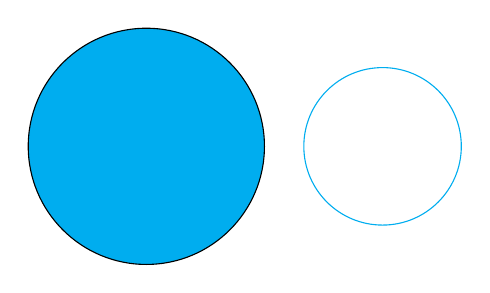
\begin{tikzpicture}
        \draw [fill=cyan, radius=1.5] (0,0) circle ;
        \draw [cyan, radius=1] (3,0) circle ;
      \end{tikzpicture}
    \end{block}

    \pause

    \begin{block}{}
      El punto de origen igual se incluye por la caracterización de
      conmutatividad del grupo fundamental y tratamiento mas explicito con
      respecto a la teoría de cubrimientos.
    \end{block}
  \end{frame}

  % Seccion ejemplo R^2 sin punto
  \begin{frame}
    \frametitle{Ejemplo intuitivo \(R^2\) menos un punto}
    \begin{figure}[h]
      \centering
      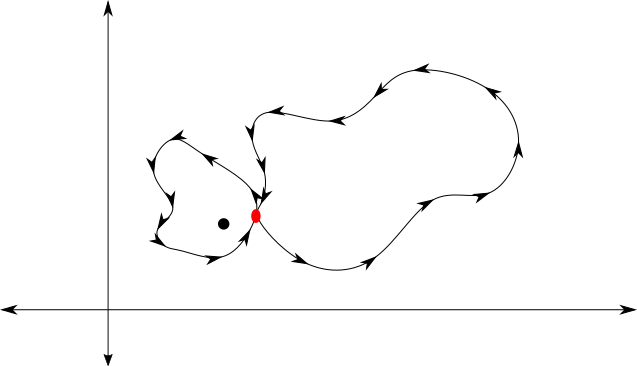
\includegraphics[scale=0.5]{../tesis/imagenes/R2-punto.png}
      \caption{\(R^2\) sin el punto \((1,1)\) en negro. Origen en rojo. }
    \end{figure}

  \end{frame}

  \begin{frame}
    \frametitle{El grupo fundamental es una invariante}
    Si \(f : (X, x) \to (Y, y) \) es un homeomorfismo, \[¿\pi (X, x)
    \simeq \pi (Y,y)?\]

    \pause

    Si, se define un isomorfismo por
    \begin{align*}
      f_* : \pi (X,x) &\to \pi (Y, y) \\
      [\gamma] &\longmapsto [ f \circ \gamma ]
    \end{align*}
  \end{frame}

  \begin{frame}
    \frametitle{Functor entre categorías}
    Lo que hemos hecho realmente con la construcción anterior es definir
    un functor \(\pi\) entre las categorías \(\mathscr{Top}_*\) y
    \(\mathscr{Grp}\)
    \[ \pi : \mathscr{Top}_* \to \mathscr{Grp} \]
    \[ \pi (f \circ g) = f_* \circ g_* \]
    \begin{center}
      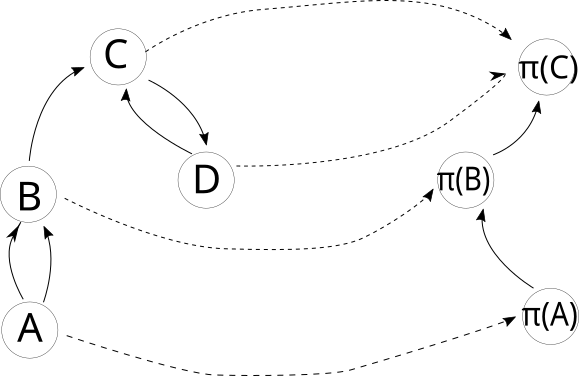
\includegraphics[scale=0.4]{./imag/categoria.png}
    \end{center}
  \end{frame}
  \begin{frame}
    \frametitle{Tres grandes herramientas de calculo}
    \begin{itemize}
    \item Retracciones y tipos homotópicos
    \item Teoría de cubrimientos
    \item Teorema de \vank
    \end{itemize}
  \end{frame}

  \begin{frame}
    \frametitle{Tipos homotópicos}
    \begin{block}{Equivalencias homotópicas}
      Sean \(f : X \to Y\) e \(g : Y \to X\) mapeos continuos. Supongamos
      que \[ g \circ f \simeq Id : X \to X \]
      \[ f \circ g \simeq Id : Y \to Y \]
      Entonces \(f\) y \(g\) son llamadas \emph{equivalencias
      homotópicas} y la presencia de estas dicen que \(X,Y\) poseen el
      mismo grupo fundamental.
    \end{block}

  \end{frame}
  \begin{frame}
    \frametitle{Lemas necesarios}
    \begin{block}{Lema}
      Si \(f \circ g = h\) con \(h\) una función biyectiva, entonces
      \(f\) sobreyectivo y \(g\) inyectivo.
    \end{block}
    \begin{block}{Lema}
      Si \(f \circ g \simeq Id\) mediante la homotopía \(H\) y \(f \circ
      g (x_0) = x_1\) entonces existe una curva \(\alpha : I \to X\)
      definida por \(\alpha (t) := H (x_0 , t)\) tal que
      \[ \hat \alpha \left( [m] \right) := [ \overline \alpha] * [m] * [\alpha]\]
      es un isomorfismo de grupo \(\pi(X,x_0) \to \pi (Y,y_0)\) y cumple
      la igualdad
      \[ f_* \circ g_* = \hat \alpha \circ Id \]
    \end{block}
  \end{frame}

  \begin{frame}
    \frametitle{Idea de demostración teorema de tipos}
    \begin{center}
      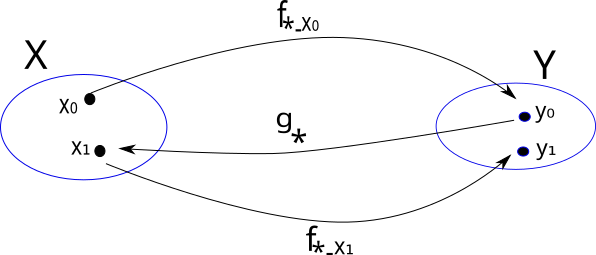
\includegraphics[scale=0.5]{./imag/teo_tipos.png}
    \end{center}
    \begin{gather*}
      f_{*,x_0} : \pi (X, x_0) \to \pi (Y, y_0) \\
      g_* : \pi (Y, y_0) \to \pi (X, x_1) \\
      f_{*,x_1} : \pi (X, x_1) \to \pi (Y, y_1)
    \end{gather*}
  \end{frame}

  \begin{frame}
    \frametitle{Ejemplo de espacios mismo tipo homotópicos}
    \begin{block}{}
      \centering
      
\includegraphics{./imag/ThreeNonHomeoButHomotopyEquivGraphs.png}
    \end{block}

    \begin{block}{}
      \centering
      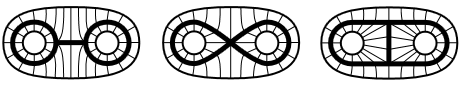
\includegraphics[scale=0.5]{./imag/HomotopyEquivalentsToBiAnnulus.png}
    \end{block}
    \begin{center}
      \emph{imágenes de Hatcher}
    \end{center}

  \end{frame}

  \begin{frame}
    \frametitle{Banda de Mobius}
    \begin{columns}
      \begin{column}{0.3\textwidth}
        \begin{center}
          \includegraphics[scale=0.2]{./imag/512px-MöbiusStripAsSquare.svg.png}
        \end{center}
      \end{column}
      \begin{column}{0.7\textwidth}
        Presentación de Banda de Mobius
        \[ M := I \times I / \{(x,1) \sim (1 - x, 0)\}\]
        \pause
        Homotópicamente equivalente a
        \begin{gather*}
          L := \{ (\frac 1 2, y) \mid y \in I \} / \{ (\frac 1 2 , 1)
          \sim (\frac 1 2, 0)\}
        \end{gather*}
        por las funciones
        \begin{gather*}
          \begin{matrix}
            r : M \to L & j : L \to M \\
            [(a,b)] \mapsto [(\frac 1 2 , b)] & [(a,b)] \mapsto [(a,b)]
          \end{matrix} \\
          r \circ j \equiv Id : L \to L, \quad j \circ r \simeq Id : M \to M
        \end{gather*}
      y \(L\) homeomorfo a \(S^1\). Luego
      \[ \pi (M) \simeq \pi (L) \simeq \pi (S^1) \]
      \end{column}
    \end{columns}
  \end{frame}

  \begin{frame}
    \frametitle{Categoría de homotopías}
    Se define una categoría \(\mathscr{HoTop}_*\) correspondiente
    a la tripleta \(\left( \mathbf{Obj}, \mathbf{Mor}, (\circ) \right)\)
    con
    \begin{itemize}
    \item \(\mathbf {Obj}\) conjunto de espacio topológicos puntuados.
    \item \(\mathbf{Mor}\) dada por el conjunto
      \begin{align*}
        \{ [f] \mid f : (X,x_0) \to (Y,y_0) \text{ continua} ,(X,x_0),(Y,y_0) \in \mathbf {Obj}\}
      \end{align*}
      de clases equivalencias homotópicas entre funciones continuas.
    \item \((\hat \circ)\) composición de clases de
      equivalencias tal que si \([f] , [g] \in \mathbf {Mor} \) con
      dominio y recorridos compatibles
      \[ [f] \hat \circ [g] = [f \circ g]\]
    \end{itemize}
  \end{frame}
  \begin{frame}
    \frametitle{Categoría de homotopías}
    \begin{block}{Subcategoría Top}
      La categoría \(\mathscr{Top}_*\) se puede ver como una
      sub-categoría de \(\mathscr{HoTop}\) mediante el functor
      \[ i : \mathscr{Top}_* \to \mathscr{HoTop}_*\]
      mapeando los objetos a si mismos y tomando toda función continua
      \(f\) entre espacios vectoriales y asignándole \([f]\) en
      \(\mathscr{HoTop}_*\).

      Espacios topológicos homeomorfos tiene claramente un par de
      equivalencias homotópicas.

      Se puede extender el functor \(\pi\) que asigna el grupo
      fundamental a un espacio topológico a trabajar desde
      \(\mathscr{HoTop}_* \to \mathscr{Grp}\)

      Muestra que la noción de homeomorfismos era muy fuerte si la meta
      es clasificar espacios mediante el grupo fundamental.
    \end{block}
  \end{frame}

  \begin{frame}
    \frametitle{Pequeñas propiedades de esta categoría}
    \begin{columns}
      \begin{column}{0.6\textwidth}
        \begin{block}{Productos}
          Es una categoría cartesiana. El producto de espacios puntuados
          sera el producto cartesiano usual \((X \times Y, (x_0, y_0))\).
          Mas aun, el functor \(\pi\) respetara la estructura del
          producto
          \[ \pi (X \times Y , (x_0, y_0)) = \pi (X, x_0) \times \pi (Y,
            y_0)\]
          siendo en la llegada el producto cartesiano de
          grupos. Este resultado se obtiene por la caracterización de
          curvas es un espacio producto.
        \end{block}
      \end{column}
      \begin{column}{0.4\textwidth}
        \begin{center}
          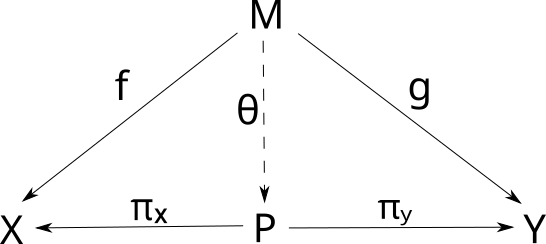
\includegraphics[scale=0.32]{../tesis/imagenes/producto.png}
        \end{center}
      \end{column}
    \end{columns}
  \end{frame}
  \begin{frame}
    \frametitle{Pequeñas propiedades de esta categoría}
    \begin{columns}
      \begin{column}{0.6\textwidth}
        \begin{block}{Co-productos}
          También tiene un co-producto por ser los objetos espacios
          puntuados. Para \((X, x_0) , (Y, y_0)\) se define el
          co-producto como
          \[ X \vee Y , \{x_0, y_0\} = X \sqcup Y / x_0 \simeq y_0 \]
          ¿Preservara \(\pi\) la estructura del co-producto?
        \end{block}
      \end{column}
      \begin{column}{0.4\textwidth}
        \begin{center}
          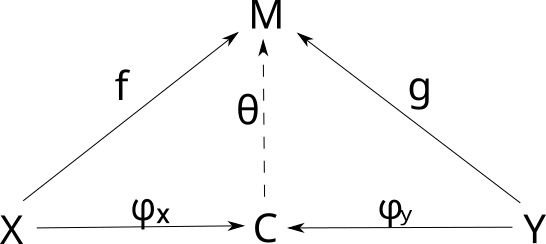
\includegraphics[scale=0.32]{../tesis/imagenes/coproducto.png}
        \end{center}
      \end{column}
    \end{columns}
  \end{frame}

  \begin{frame}
    \frametitle{Cubrimientos}
    \begin{columns}
      \begin{column}{0.3\textwidth}
        \centering
        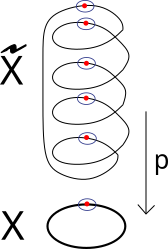
\includegraphics[scale=.8]{../tesis/imagenes/spring.png}
      \end{column}
      \begin{column}{0.7\textwidth}
        \begin{block}{Cubrimiento}
          \(p : \tilde{X} \to X\) una función continua sobreyectiva tal
          que para todo \(x \in X\) existe un abierto U y una familia
          \(\{V_\alpha\}_{\alpha \in \Lambda},\ \Lambda \subseteq \mathbb N\) tal
          que
          \[ p^{-1} (U) = \bigcup_{\alpha \in \Lambda} V_\alpha \]
          Donde \(\{V_\alpha\}\) es una familia disjunta de abiertos de
          \(\tilde X\), tal que
          la restricción a cada \(V_\alpha\) de \(p\) es
          homeomorfa sobre \(U\).
        \end{block}
        \begin{block}{Fibra}
          Corresponde al conjunto de puntos en rojo.
          \[ p^{-1} \left( \{x_0\} \right) \]
        \end{block}
      \end{column}
    \end{columns}
  \end{frame}

  \begin{frame}
    \frametitle{Levantamiento de curvas al cubrimiento}
    \begin{columns}
      \begin{column}{.4\textwidth}
        \centering
        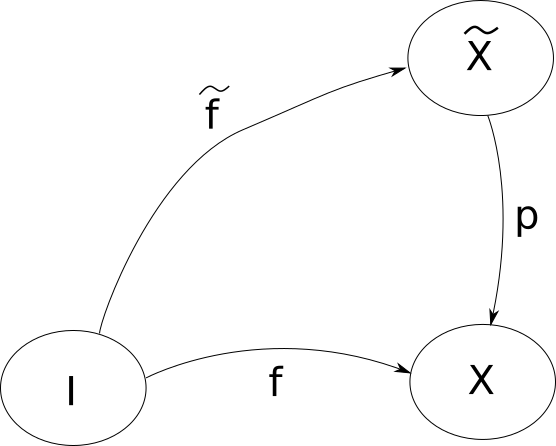
\includegraphics[scale=0.3]{../tesis/imagenes/lifting-path.png}
        \[ p \circ \tilde f = f \]
      \end{column}
    \begin{column}{.6\textwidth}

      \begin{block}{Levantamiento de caminos}
        Sea \(p : \tilde X \to X\) un cubrimiento y \(x_0 \in X\).
        Fijemos algún \(\tilde x _0 \in p^{-1} \{x_0\} \subset \tilde
        X\). Para cualquier camino \(f : [0,1] \to X\) que comience en \(x_0\),
        existe un único camino levantamiento \(\tilde f : [0,1] \to \tilde X\)
        tal que \(\tilde f (0) = \tilde x _0\)
      \end{block}

      \pause

      \begin{block}{Levantamiento de homotopías}
        Sea \(p : \tilde X \to X\) un cubrimiento par tal que \(p(\tilde
        x _0) = x_0 \) para algún \(\tilde x _0 \in \tilde X\). Para cualquier
        función continua \(F : I \times I \to X\) tal que \(F(0,0) = x_0\),
        tiene una única función levantamiento continua \(\tilde F : I \times I
        \to \tilde X\) que cumpla \(\tilde F (0,0) = \tilde x_0\)
      \end{block}
    \end{column}
    \end{columns}
  \end{frame}

  \begin{frame}
    \frametitle{inyectividad cubrimientos}
    \begin{block}{}
      Sea \(\left( \tilde X, \tilde x_0 \right), \left( X, x_0 \right)\)
      dos espacios topológicos puntuados. Si \(p : \left( \tilde X,
        \tilde x_0 \right) \to \left( X, x_0 \right)\) un cubrimiento
      entre estos, entonces el homomorfismo inducido
      \[ p_* : \pi \left( \tilde X, \tilde x_0 \right) \longrightarrow
        \pi \left( X, x_0 \right)\] es inyectivo.
    \end{block}
  \end{frame}

  \begin{frame}
    \frametitle{Cubrimiento universal}
    \begin{block}{Cubrimiento universal}
      Un cubrimiento universal \(p : \tilde X \to X\) es tal que \(\pi
      (\tilde X, \tilde x_0) = \{e\}\).
    \end{block}

    \begin{block}{Levantamiento derivado}
      Si \(p : \tilde X \to X\) es un cubrimiento con \(\tilde X\)
      universal, entonces para todo \(\tilde x_0 \in p^{-1} (x_0)\) se
      puede definir una función biyectiva
      \[ \phi : \pi (X, x_0) \to p^{-1} (\{x_0\}) \]
      \[ \phi \left( [f] \right) = \tilde f (1) \]
    \end{block}
  \end{frame}

  \begin{frame}
    \frametitle{Ejemplos}
  \begin{columns}
    \begin{column}{0.5\textwidth}
      \(\pi (S^1,x_0)\) es isomorfo a \((\mathbb Z, +)\) \\
      \centering
      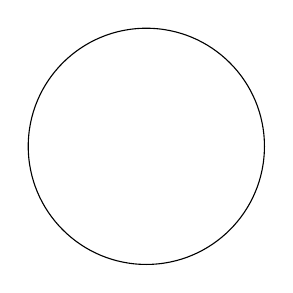
\begin{tikzpicture}
        \draw (0,0) circle [radius=1.5];
      \end{tikzpicture}
    \end{column}

    \begin{column}{0.5\textwidth}
      \(\pi (RP^2, x_0)\) es isomorfo a \(\mathbb Z / 2 \mathbb Z\) \\
      \centering
      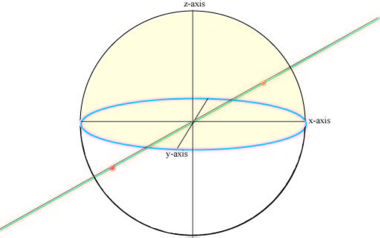
\includegraphics[scale=0.5]{./imag/rpsphere.jpg}
    \end{column}
  \end{columns}
  \end{frame}

  \begin{frame}
    \frametitle{Caracterización de functor}
    \begin{block}{}
      Se define una nueva categoría de cubrimientos de espacios \(X\)
      que posean cubrimiento universal. Luego se define un functor
      \(\pi\) el cual mapea elementos iniciales de \(\mathscr{Cov}\) a
      el grupo trivial (elemento inicial) de \(\mathscr{Grp}\) y donde
      los morfismos pasan a ser inyecciones de grupos
    \end{block}
    \begin{block}{}
        \centering
        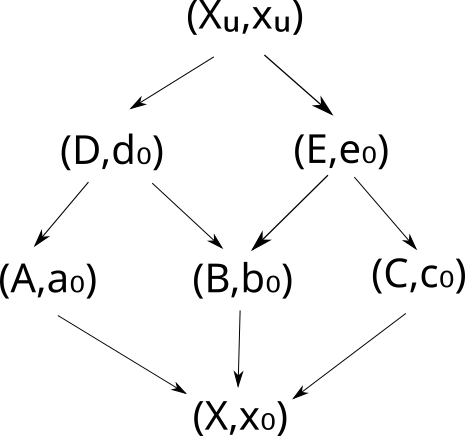
\includegraphics[scale=0.3]{../tesis/imagenes/cov.png}
      \end{block}
  \end{frame}

  \begin{frame}
    \frametitle{\vank}
    \begin{block}{\vank}
      Sea \(X = U \cup V\), donde \(U,V\) son conjuntos abiertos de \(X\).
      Supongamos que \(U \cap V\) es arco-conexo y que \(x_0 \in U \cap V\).
      Sea \(j_1\) y \(j_2\) las inclusiones de \(U\) y \(V\) en \(X\)
      respectivamente. Entonces las imágenes de los homomorfismos inducidos
      \[ j_{1,*} : \pi (U, x_0) \to \pi (X, x_0), \quad j_{2,*} : \pi
      (V, x_0) \to \pi (X, x_0) \]
      generan a \(\pi (X,x_0)\).

      \begin{center}
        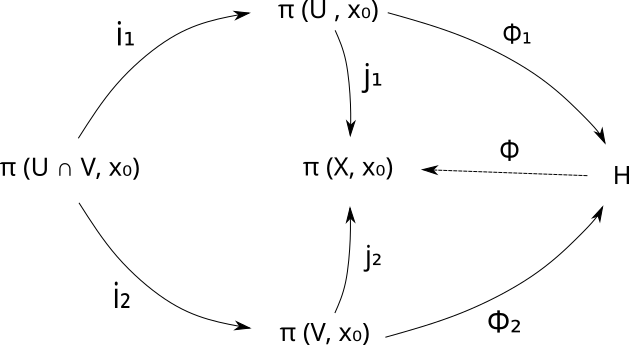
\includegraphics[scale=.35]{../tesis/imagenes/van.png}
      \end{center}
    \end{block}
  \end{frame}

  \begin{frame}
    \frametitle{Ejemplos \(S^1 \vee S^1\)}
    \begin{center}
      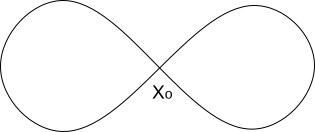
\includegraphics[scale=0.4]{../tesis/imagenes/figura8.png}
    \end{center}
    \pause
    Notar que para todo \(x_0\) existe una vecindad contractible \(U_x\)
    se este. Luego
    \[ A_1 = S^1 \vee U_x , \quad A_2 = U_x \vee S^1 \]
    \[ \implies A_1 \cup A_2 = (S^1 \vee S^1, x_0) , \quad A_1 \cap A_2 = (U_x , x_0) \]
    con \(\pi (U_x , x_0)\) trivial. Luego
    \[ \pi (S^1 \vee S^1) = \pi (S^1) * \pi (S^1) \text{ por \vank}\]
    \pause
    Solo se preservan co-productos de espacios semi-localmente
    simplemente conexos mediante \(\pi\)
  \end{frame}

  \begin{frame}
    \frametitle{Botella Klein}
    \begin{center}
      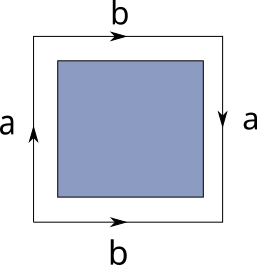
\includegraphics[scale=0.3]{../tesis/imagenes/kleinU.png}
      \hspace{3mm}
      
\includegraphics[scale=0.3]{../tesis/imagenes/kleinV.png}
      \hspace{3mm}
      
\includegraphics[scale=0.3]{../tesis/imagenes/kleinUV.png} \\
      \hspace{2mm} \(U\) \hspace{19mm} \(V\) \hspace{16mm} \(U \cap V\)
    \end{center}
    \pause
    \begin{gather*}
      \pi (U) = \{e\}, \quad \pi (V) = \{[e], [a], [b]\} \\
      \pi (U \cap V) = \{[\gamma], [e]\} \text{ se retrae a } S^1 \\
      i_{u,v} ([\gamma]) = [e], \quad i_{v,u} ([\gamma]) = [\gamma]_V
    \end{gather*}
    Pero \([\gamma]_{V} = [a]*[b]*[a]*[b^{-1}] \) por homotopía
    radial. Luego
    \[ N \left( \{[a]*[b]*[a]*[b^{-1}]\} \right) = \{[a]*[b]*[a]*[b^{-1}]\} \]
    \[ \pi (U \cup V) = \langle [a], [b] \rangle /
      \{[a]*[b]*[a]*[b^{-1}] = e\}\]
  \end{frame}

  \begin{frame}
    \frametitle{Pushout por \vank}
    \begin{center}
      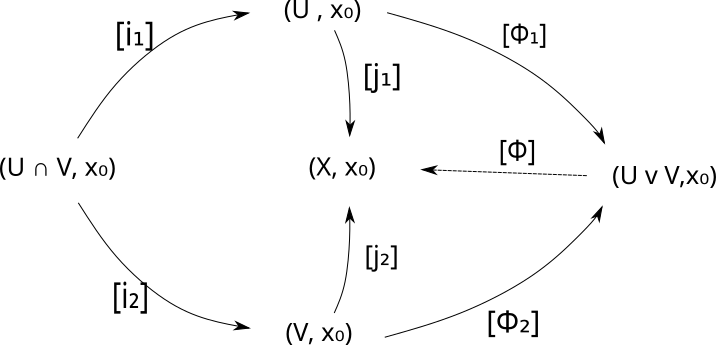
\includegraphics[scale=0.33]{../tesis/imagenes/pushoutHotop.png}
    \end{center}
  \end{frame}
\end{document}
